%%%%%%%%%%%%%%%%%%%%%%%%%%%%%%%%%%%%%%%%%%%%%%%%%%%%%%%%%%%%%%%%%%%%%%%%%%%%%%%

\chapter{METHOD}\label{ch:prop}

In this section, the objectives will be reviewed, the case study data will be presented and also the proposed architecture.

\section{Objectives}\label{ch:prop:obj}

Recalling from \autoref{ch:intro:obj}, the main objective of this thesis is to "create a data cube base architecture to represent satellite telemetry data along a mission, using the distribution of the telemetry values to ease analysis and querying of the satellite's state by satellite engineers".
In order to achieve that, and as specific goals, two different architectures will be proposed and implemented: one tries to reduce main memory consumption by pre-processing the data to be queried into high-dimensional and low-dimensional, and then filters the resulting data cubes by the dimensions related to each pre-defined query; the other uses an inverted index compression technique of changing the TID lists to hold interval lists instead of raw number lists, and tries to see how that affects query response time and memory consumption.

\section{Case Study: SCD2}\label{ch:prop:scd2}

The case study used in this thesis will be the satellite SCD2 (Data Collection Satellite in Portuguese), which has over 20 years of continuous operations by the Satellite Control Center at INPE~\cite{OrlandoKuga:2007:SaSCSC}.
It is one of the first satellites designed, tested and assembled in Brazil, the second in the SCD family of data collection satellites~\cite{Oliveira:1996:SC1Sa}.
The mission goal is to retransmit to assigned receiver stations (Cuiabá and Alcântara, for example), data obtained from a network of Automatic Environmental Data Collection Platforms (PCD), which are distributed throughout the Brazilian territory.
\autoref{fig:scd2_mission} shows a commemorative mission patch for the satellite.

Each PCD is composed of a transmitter in UHF band (about $400Mhz$) that collects environmental data and continuously transmits them back into space.
This transmission is then relayed by the PCD transponder to one of the receiver stations, and thus the data is gathered.
This relaying can only happen when the satellite is visible by both the receiver stations and the PCDs, which happens around eight times per day~\cite{miguezSCD2OperationHandbook1993}.

The SCD2 satellite is composed of ten subsystems, including the DCP payload.
With over 20 years of operation, more than 135 telemetry data points and generating over 8GB of data per year, there is a lot to be analyzed from the housekeeping telemetry data alone.
This work has access to data taken between 2014 and 2018, and amounts to about 23GB of CSV files.
These data were obtained by exporting the telemetry database to CSV format via the SatCS program developed at INPE~\cite{azevedoFRAMEWORKSISTEMACONTROLE2015}, taking over three weeks to process the data.

\begin{figure}[H]
  \caption{SCD2}\label{fig:scd2_mission}
  \vspace{6mm}
  \begin{center}
    \resizebox{5cm}{!}{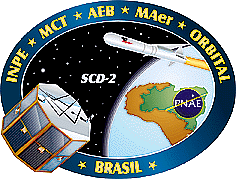
\includegraphics{Figuras/Scd-2.png}}
  \end{center}
  \vspace{2mm}
  \legenda{Data Collection Satellite 2 (SCD2) mission patch}
  \FONTE{Taken from \url{http://www.inpe.br/noticias/galeria/}}
\end{figure}

\section{Proposed Architecture}\label{ch:prop:static}

One of the using necessities of different data cube algorithms is in the number of dimensions that a certain cube can perform queries: queries with more than 15 dimensions are not generally (or practically) executed in some algorithms, as the work of~\citeonline{silvaComputingBIGData2016} demonstrates, however demonstrating some works that do execute queries with more dimensions than that.

The telemetry data of interest has many more dimensions than the common limit for data cube with up to 60 dimensions: with over 135 telemetries for the SCD family satellites, and thousands for larger satellites like CBERS and Amazonia, running high-dimensional queries would typically be infeasible in traditional cube construction algorithms.

It is then needed to first propose an overall architecture that takes the data from input, processes it and then spits out an analysis on the other side.
This is presented as a data cube answering queries, after having been inputed sufficient data and statistical information about this data.
An overview of this architecture is present in \ref{fig:architecture_static}, showing how the data is based on databases
The figure~\ref{fig:architecture_static} shows an overview of the proposed structure.
The biggest gain of using the data cube is, plainly, to easily execute group-by operators on multiple aggregation levels and using multiple dimensions at once to compute the relationship measures between them.

In this figure, the Frag-Cubing algorithm has been arbitrarily divided into the steps of reading the input, building the inverted index, building the shell fragments in accord to the algorithm and then the cubing step that generates the data cube aggregations and is shown in the middle of the picture.
The users can then query into this structure via a Query Processor built-in.

\begin{figure}[!htb]
  \caption{General Data Cube Architecture}\label{fig:architecture_static}
  \vspace{2mm}
  \begin{center}
    \resizebox{15cm}{!}{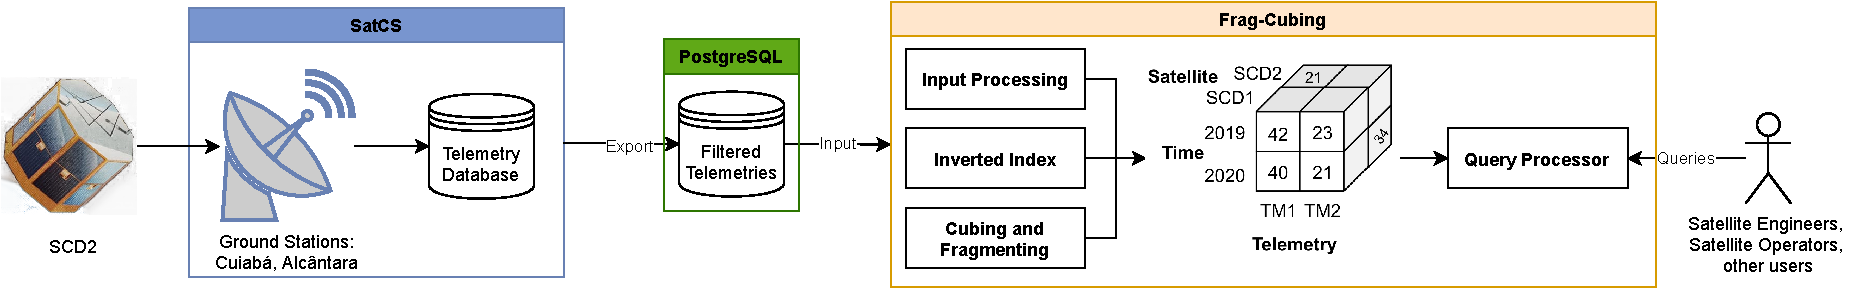
\includegraphics{Figuras/Static_Structure.pdf}}
  \end{center}
  \vspace{1mm}
  \legenda{Data Cube-based architecture showing the data being generated by the satellite, being processed by SatCS, exported to a raw CSV format into PostgreSQL, which is then used as a Data Warehouse base to build a Data Cube using the Frag-Cubing algorithm. The user can then query the data cube directly.}
  \FONTE{Author}
\end{figure}

\subsection{Proposed changes}\label{ch:prop:static:dynamic}

In order to achieve the objectives of this thesis, the following changes are then proposed, illustrated by~\autoref{fig:architecture_dynamic}: change the Frag-Cubing algorithm into the IntervalFrag algorithm by changing the inverted index step into an inverted index with intervals; add the Query Partition step in which the telemetry value distribution is used to filter out relationships between the telemetries with the help of a Satellite Engineer, and have those relationships influence what data is then input into IntervalFrag.
The overall objective is to show that only some changes are made into the Frag-Cubing algorihtm, and the Query Partition is an added optional step.
The changes have been highlighted in red lettering.

\begin{figure}[!htb]
  \caption{General Data Cube Architecture}\label{fig:architecture_dynamic}
  \vspace{2mm}
  \begin{center}
    \resizebox{13cm}{!}{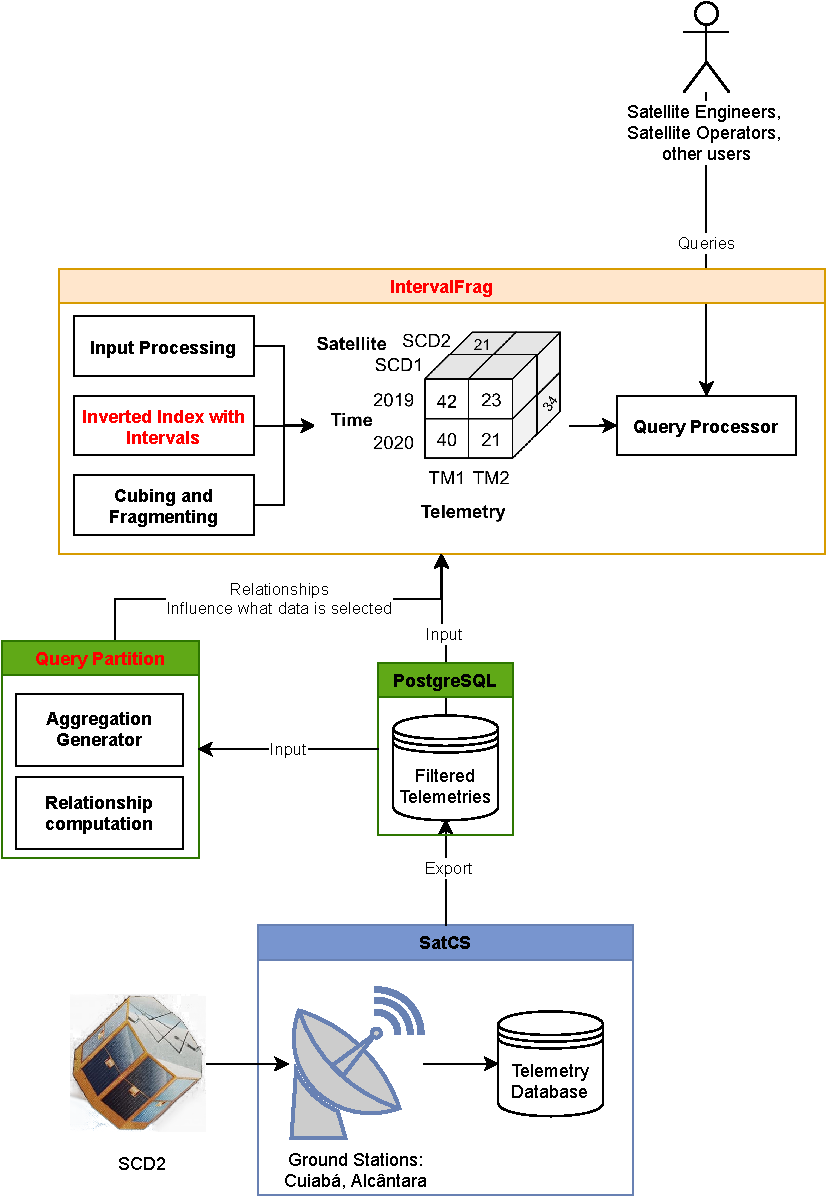
\includegraphics{Figuras/Dynamic_Structure.pdf}}
  \end{center}
  \vspace{1mm}
  \legenda{Data Cube-based architecture showing the data being generated by the satellite, being processed by SatCS, exported to a raw CSV format into PostgreSQL, which is then used as a Data Warehouse base to build a Data Cube using the IntervalFrag algorithm.
    The Query Partition algorithms can then use the information obtained from the data to filter out dimensions to be input into IntervalFrag.
  The user can then query the data cube directly, or the relationships if necessary.}
  \FONTE{Author}
\end{figure}

In the next chapters, the Query Partition algorithm will be presented and the results of using the approach will be shown, then the IntervalFrag algorithm will be explained, the constituent algorithms that diverge from Frag-Cubing explained and the experimental results shown.

%\RED{How to describe the architecture and the data how Mauricio detailed it? I guess this is the best option}
%- Como objetivo específico ou adicional, como o uso do IntervalFrag no Frag-Cubing
%- Colocar o mesmo desenho da arquitetura com a camada do Frag-Cubing, isso é para explicar a arquitetura alto nível, e uma arquitetura dinâmica de como funciona o Frag-Cubing/meu trabalho.
%- Pensar nas camadas, montar um framework para transformar os dados de telemetrias em um cubo de dados para facilitar as consultas, inclusive como forma de melhorar o desempenho
%- Utilizar aquele projeto do R para visualizar, mostrar como os dados são mostrados, onde entram e o que mostram
%- Utilizar como base aquela arquitetura DOTNET em camadas? -> Uma arquitetura mais rebuscada, com mais cores (???), dorar a pílula como se fosse para ganhar dinheiro
%- Utilizar um fluxograma para representar a dinâmica dessa arquitetura
%- Criar uma arquitetura em nível mais alto e fazer as chamadas para a arquitetura -> Não entende em qual contexto da arquitetura o Interval entra
%- O quê se ganha com a representação em cubo de dados -> Forma melhor de executar consultas com group-by, isso é um ganho para o trabalho -> Colocar isso na contribuição

